\section{Arithmetic classification of collective regimes}\label{sec:regimes}
The collective map is organised by the \emph{class number} $G(x)$. Two facts from \cref{lem:basic} drive everything: $b\mid G$, and $G(C(x))\mid G(x)$ because $D(x)\subseteq D(C(x))$ (\cref{lem:M}) and a gcd over a larger set divides the gcd over a smaller one. Hence $G_n=G(x_n)$ is eventually constant, with limit $G_\infty$, along any orbit with $D(x_0)\ne\emptyset$. We distinguish \emph{regime I} ($G=1$, integer states), \emph{class orbits} ($G=b>1$, fixed denominator) and everything else.

\subsection{Regime I: integer states with \texorpdfstring{$G=1$}{G=1}}
For an integer $m$ with $\sigma=\sigma(m)>1$ write $m=t\sigma^2$; then $t=\prod_pp^{\varepsilon_p}$ with $\varepsilon_p=v_p(m)-2q_p\in\{0,1\}$ is squarefree. Moreover $D(m)$ is the set of non-trivial divisors of $\sigma$, so $L=\sigma$.

\begin{theorem}[regime-I reduction and the rigid set]\label{thm:B2T6}
Let $m=t\sigma^2$ be as above with $G(m)=1$. Then $C(m)=(t+1)\sigma^2=t'(\sigma u)^2$ with $t'=\sqf(t+1)$ the squarefree part and $u^2=(t+1)/t'$; $G(C(m))=1$ and $\sigma(C(m))=\sigma u$. The pair $(\sigma,t)$ therefore evolves by
\[
(\sigma,t)\longmapsto(\sigma u,\ \sqf(t+1)),\qquad u=\sqrt{(t+1)/\sqf(t+1)} .
\]
The set $\{t=1,2,3\}$ is invariant, with $(\sigma,1)\to(\sigma,2)\to(\sigma,3)\to(2\sigma,1)$; on it $C^3(m)=4m$. Every orbit enters it, and the only cycle of the $t$-map $t\mapsto\sqf(t+1)$ is $(1,2,3)$.
\end{theorem}
\prov{CW-0400}{B2-T6}{PROVED}{FULL}
\begin{proof}
Since $G=1$ we have $C(m)=m+\sigma^2=(t+1)\sigma^2$. Writing $t+1=t'u^2$ gives the displayed form and $\sigma(C(m))=\sigma u$ (the $t'$ part is squarefree). By \cref{lem:basic}, $G(C(m))\mid G(m)=1$. The three steps for $t\in\{1,2,3\}$ follow from $\sqf(2)=2$, $\sqf(3)=3$, $\sqf(4)=1$ with $u=2$ at the last step; hence $C^3(\sigma^2)=4\sigma^2$, and likewise for $2\sigma^2,3\sigma^2$.

\emph{Descent.} Let $t\ge4$ be squarefree and write $t_0=t$, $t_{j+1}=\sqf(t_j+1)$. As long as $t_j+1$ is squarefree, $t_{j+1}=t_j+1$. Among $t+1,\dots,t+4$ one number is divisible by $4$, hence not squarefree; so there is a first $j\le3$ with $t+j+1$ not squarefree, and then $t_{j+1}=\sqf(t+j+1)\le(t+j+1)/4\le(t+4)/4<t$. Thus within four steps the value of $t$ drops strictly below its starting value, and by induction on $t$ every orbit reaches $t\le3$, i.e. the set $\{1,2,3\}$ of squarefree values below $4$. A cycle other than $(1,2,3)$ would contain its minimum $t_*\ge4$ and would then have to drop below $t_*$, a contradiction. \qedhere
\end{proof}
\begin{remark}[entry times; finite-exact]\label{rem:entry}
The entry time into $\{1,2,3\}$ depends only on $t$. For all squarefree $t<3000$ the maximum number of applications of $t\mapsto\sqf(t+1)$ needed is $12$ (attained at $t=1301$); the identity $C^3(m)=4m$ was also confirmed for $90$ integers of the rigid domain (\stat{finite-exact}).
\end{remark}

\subsection{Eventual rigidity: the corrected statement}
\begin{definition}[rigid]\label{def:rigid}
An orbit is \emph{rigid} if $x_{n+3}=4x_n$ for all large $n$, i.e.\ it has period $3$ with multiplier $4$ (the case of the rigid set above).
\end{definition}
\begin{proposition}[eventual rigidity; B2-T7, corrected]\label{prop:B2T7}
\begin{enumerate}[label=(\alph*),itemsep=1pt]
\item If $G_\infty=1$, the orbit is eventually an integer orbit of regime~I and is eventually rigid; the entry time after the first index with $G_n=1$ depends only on the value of $t$ at that index.
\item The converse is false: there are rigid orbits with $G_\infty=5$ (the tower of \cref{thm:R3T5c}).
\end{enumerate}
Consequently ``rigidity $\Leftrightarrow G_\infty=1$'' is not a theorem; the correct statement is \emph{only} $G_\infty=1\Rightarrow$ rigidity.
\end{proposition}
\prov{CW-0401}{B2-T7}{CORRECTED}{CORRECTED}
\begin{proof}
(a) If $G_\infty=1$ then $G_N=1$ for some $N$, hence $b_N\mid G_N=1$ and $x_N$ is an integer with $\sigma(x_N)>1$ (as $D\ne\emptyset$); \cref{thm:B2T6} applies from $N$ on. (b) is \cref{thm:R3T5c}. \qedhere
\end{proof}
\begin{remark}[provenance of the correction]
The earlier wording of this item asserted ``rigid iff $G_\infty=1$''. The $G=5$ tower of \cref{sec:towers} shows that the implication from rigidity to $G_\infty=1$ is false; the forward implication is proved above and agrees with the inherited statement (FIELD-I, Thm.~32 of~\cite{FoundII}).
\end{remark}
\Cref{fig:coords} plots the collective coordinates along an orbit.
\begin{figure}[tbp]\centering
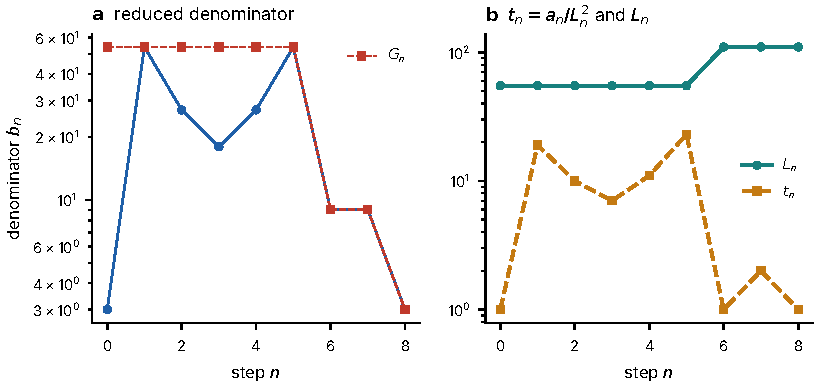
\includegraphics[width=\textwidth]{fig06_collective_coordinates}
\caption{\textbf{Collective coordinates along an orbit (exact; finite-exact data of \cref{sec:activation}).} The eight-step orbit $3025/3\to12100/3$ (parameters: $x_0=3025/3$, $n=0..8$). (a) reduced denominator $b_n$ and $G_n$ (log scale); $b_n\mid G_n$ at every step. (b) $L_n$ and $t_n=a_n/L_n^2$. Abstract quantities ($G,t$) and geometric ones ($L$) are shown together; no extrapolation.}\label{fig:coords}
\end{figure}
\begin{figure}[tbp]\centering
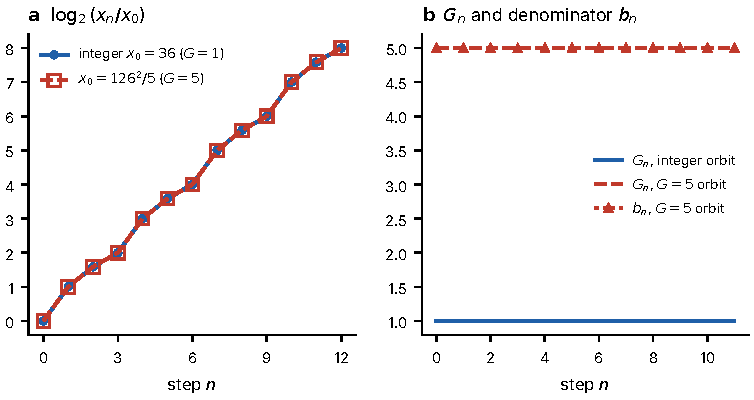
\includegraphics[width=\textwidth]{fig07_rigid_vs_persistent}
\caption{\textbf{Rigid orbits with $G=1$ and $G=5$ (finite-exact; the pattern is proved by \cref{thm:B2T6,thm:R3T5c}).} (a) $\log_2(x_n/x_0)$ for the integer orbit $x_0=36$ and for $x_0=126^2/5$, $n\le12$: both advance by $2$ every three steps, so the two curves coincide (the second is drawn with hollow markers). (b) $G_n$ for both orbits and the denominator of the second: $G$ equals $1$ resp.\ $5$ throughout, which is why rigidity does not force $G_\infty=1$.}\label{fig:rigid}
\end{figure}

\subsection{The class \texorpdfstring{$G=b$}{G=b}}
\begin{theorem}[exact reduction in the class $G(x)=b$]\label{thm:R3T5a}
Let $x=a/b$ be reduced with $D(x)\ne\emptyset$ and $G(x)=b$. Then $L^2\mid a$, so $x=tL^2/b$ with $t\in\N$, and $C(x)=(t+1)L^2/b$. If $\gcd(t+1,b)=1$ this fraction is reduced, $D(x)\subseteq D(C(x))$ and $G(C(x))=b$; if $\gcd(t+1,b)>1$ the denominator of $C(x)$ is a proper divisor of $b$ and the orbit leaves the class. While $D$ (hence $L$) is unchanged, $t$ increases by exactly $1$ per step.
\end{theorem}
\prov{CW-0416}{R3-T5a}{PROVED}{FULL}
\begin{proof}
For every prime $p$, $v_p(L)=\max_{d\in D}v_p(d)$ and $2v_p(d)\le v_p(a)$, so $L^2\mid a$. Since $G=b$ we have $h=1$ in $C(x)=(ah+L^2)/G$, giving $C(x)=(a+L^2)/b=(t+1)L^2/b$. By \cref{lem:basic}, $\gcd(L,b)=1$ (as $\gcd(L,G)=1$), so reducedness is equivalent to $\gcd(t+1,b)=1$. In that case $b\mid G(C(x))$ (basic fact for the reduced denominator $b$) and $G(C(x))\mid G(x)=b$ (monotonicity), hence equality. Otherwise cancelling the common factor shrinks the denominator. \qedhere
\end{proof}
\begin{theorem}[first event of a fresh stage; dichotomy, $b=\ell$ prime]\label{thm:R3T5b}
Let $\ell$ be prime and $x=L^2/\ell$ with $G(x)=\ell$ and $L=\lcm D(x)$ (a \emph{fresh stage}, $t=1$); write $D_\ell(S)=\{d\mid S:d\ge2,\ d\equiv1\ (\ell)\}$, so that $D(x)=D_\ell(L)$.
\begin{enumerate}[label=(\alph*),itemsep=1pt]
\item Put $u^*=\min\{u\ge2:D_\ell(uL)\ne D_\ell(L)\}$. As long as $u^{*2}<\ell$, the set $D$ is unchanged for $1\le t<u^{*2}$ and changes at $t=u^{*2}$; the stage has length $u^{*2}-1$. If $u^{*2}>\ell$ the orbit reaches the integer $L^2$ first and leaves the class.
\item Dichotomy: an orbit in the class either leaves it (becoming an integer) in finitely many steps, or has infinitely many occurrence events.
\end{enumerate}
\end{theorem}
\prov{CW-0417}{R3-T5b}{PROVED}{FULL}
\begin{proof}
(a) By \cref{thm:R3T5a} the states are $x_t=tL^2/\ell$ while $D$ is unchanged. Write $t=u_t^2\tau'$ with $\tau'$ squarefree; then $a=\tau'(u_tL)^2$ and $d^2\mid\tau'(u_tL)^2$ iff $d\mid u_tL$ (at each prime $2v_p(d)\le1+2v_p(u_tL)$ forces $v_p(d)\le v_p(u_tL)$). Hence $D(x_t)=D_\ell(u_tL)$ with $u_t^2\le t$. The sets $D_\ell(uL)$ increase with $u$ under divisibility, so for $t<u^{*2}$ we have $u_t<u^*$ and $D(x_t)=D_\ell(L)$ by minimality, while at $t=u^{*2}$, $u_t\ge u^*$ and $D$ has changed. The class is left exactly when $\ell\mid t+1$, which for $t<\ell$ first happens at $t=\ell-1$; since $\ell$ is prime $u^{*2}\ne\ell$, and $u^{*2}<\ell$ means the event comes first. (b) If there are finitely many events then $D$, hence $L$, is eventually constant, $t$ increases by one at each step (\cref{thm:R3T5a}) and $\ell\mid t+1$ within $\ell$ steps: the orbit leaves the class. \qedhere
\end{proof}
\begin{remark}
The stage that follows an event is again fresh iff $\lcm D_\ell(u^*L)=u^*L$; this holds in all the towers below, where it is verified, but it is not claimed in general (\cref{sec:towers}).
\end{remark}

\subsection{Rigid strands (finite-exact)}
\begin{proposition}[ratios along rigid strands]\label{prop:BT11}
On a rigid orbit with $x_n=t_n\sigma_n^2/b$ in the sequence $t=1,2,3,\ldots$ (the cases $G=1$ and the tower $G=5$), the consecutive ratios are $x_{n+1}/x_n=2,\ 3/2,\ 4/3$ in rotation, the displacement over one period is $4=2^2$ (exponent vector $2e_2$), and the multiplicative group generated by the ratios, $\langle2,3/2,4/3\rangle=\langle2,3\rangle$, has rank~$2$.
\end{proposition}
\prov{CW-0393}{B-T11}{FINITE-EXACT}{FINITE}
\begin{proof}
In both cases $x_n=(j+1)\sigma^2/b$ with $j=n\bmod3$ and $\sigma$ multiplied by $2$ per period: this gives the ratios $2/1,3/2,4/3$ and the product $4$. The group is generated by $2$, $3/2$, $4/3$ hence contains $3$ and $2$ and equals $\langle2,3\rangle$. \qedhere
\end{proof}
\begin{remark}
The inherited statement (FIELD-I) also records that this pattern holds on all $600$ realised states of a $20{,}000$-candidate sample; that census is \stat{cited}, not re-run. The proof above covers only the two explicit families.
\end{remark}
